\section{Approximation Algorithms and Local Search Heuristics.}
\begin{itemize}
	\item \textbf{Kompleksitetsklassen} $\mathbf P$ er klassen af sprog, der kan blive besluttet i polynomiel tid af en Turing maskine
	\item \textbf{NP} er klassen af sprog $L$ hvor der eksister et sprog $L' \in \mathbf P$ og et polynomium $p$ således at
  \begin{equation*}
    \forall v: x \in L \Leftrightarrow [\exists y \in \{0,1\}^* : |y| \leq p(|x|) \land \langle x, y \rangle \in L']
  \end{equation*}
  \item Given to sprog $L_1$ og $L_2$ reducerer $L_1$ til $L_2$, hvis der er en polynomiel udregnelig funktion $r$ således at for alle $x \in \{0,1\}^*$ har at
  \begin{equation*}
    x \in L_1 \Leftrightarrow x \in L_2
  \end{equation*}
  Skrevet som $L_1 \leq L_2$ 
  \item Et sprog $L$ er et $\mathbf{NP}$ hård sprog, hvis den har den egenskab af for alle $L' \in \mathbf{NP}$, $L'$ reducerer til $L$ 
  \item Klassen $\mathbf{NPC}$ er klassen af $\mathbf{NP}$ komplette sprog, som er de sprog i $\mathbf{NP}$ som er $\mathbf{NP}$ hårde.
\end{itemize}

\subsection{Approximation algoritmer}
\begin{itemize}
	\item En approximations algoritme er en algoritme, der prøver at approximere et NP komplet problem i polynomiel tid.
  \item En algoritme for et problem har en \textbf{approximationsratio} på $p(n)$, hvis for et hvert input af størrelse $n$, pris $C$ af løsning er inden for en faktor af $p(n)$ af den optimal løsning $C^*$ 
  \begin{equation*}
    \max\bigg(\frac C{C^*} \frac{C^*}{C} \bigg) \leq p(n)
  \end{equation*}
  \item Hvis en algoritme har en approximationsratio på $p(n)$ kaldes det for en $p(n)$ approximationsalgoritme
\end{itemize}

\subsubsection{Vertex cover}
\begin{itemize}
\begin{figure}[ht]
	\centering
\begin{lstlisting}
APPROX-VERTEX-COVER(G)
  $C= \emptyset$
  $E' = G.E$
  while $E' \neq \emptyset$
    lad $(u,v)$ være en arbritær kant i $E'$ 
    $C = C \cup \{u,v\}$
    fjern fra $E'$ alle kanter til $u$ eller $v$ 
  return $C$
\end{lstlisting}
	\caption{Approximationsalgoritme til vertex cover problemet\label{fig:approx-vertex}}
\end{figure}

  \item Et \textbf{vertex cover} af en undirected graf $G=(V,E)$ er et subset $V' \subseteq V$ således at hvis $ij \in V$ så er enten $i \in V'$ eller $j \in V'$ eller begge. 
  \item \textbf{Vertex-cover} problemet er at finde et vertex cover af en minimum størrelse givet en undirected graf. Et sådan cover er kaldt et \textbf{optimal vertex cover} og problemet er et \textbf{NP} komplet problem. 
  \item \textbf{Theorem} APPROX-VERTEX-COVER (Figur \ref{fig:approx-vertex}) er en polynomiel tid 2 approximationsalgoritme for vertex cover
  \begin{proof} 
    Algoritmen kører i polynomieltid, da den kigger på være knude og hver kant en gang dvs. at den kører i $O(|V| + |E|)$ \smallskip
  
    Algoritmen finder et vertex cover siden den looper indtil alle kanter $G.E$ er blevet dækker af en af en vertex \smallskip

    For at vise at det er en 2-approximationsalgoritme lader vi $A$ være den mængde af kanter, som bliver valgt af APPROX-VERTEX-COVER. For at dække alle kanter må et optimal cover $C^*$ indeholde mindst et af punkterne fra være af kanterne. Siden ingen kanter i $A$ deler et slut punkt får vi følgende nedre grænse
    \begin{equation*}
      |C^*| \geq |A|  
    \end{equation*}
    Siden begge endepunkter af kanterne i $A$ bliver valgt får vi følgende lighed:
   \begin{equation*}
      |C| = 2|A| 
   \end{equation*}
    Ud fra disse denne lighed og ulighed får vi approximationsratio
    \begin{equation*}
      |C| = 2|A| \leq 2|C^*|
    \end{equation*}
    Dette beviser dermed theoremet

  \end{proof}
\end{itemize}

\subsubsection{The traveling-salesman problem}
\begin{figure}[ht]
    \centering
\begin{lstlisting}
APPROX-TSP-TOUR($G$,$x$)
  lad en arbritær vertex $r\in G.V$ til at være roden
  udregn et minumum spanning tree $R$ for $G$ fra roden $r$ vedhjælp af MST-PRIM($G$, $c$, $r$)
  lad $H$ være en list af kanter, der er ordnet efter hvornår de først er blevet besøg i en tree walk af $T$
  return hamiltonian cykel $H$
\end{lstlisting}
    \caption{2 Approximationsalgoritme for TSP med trekantsuligheden \label{fig:approx-tsp-tour}}
\end{figure}

\begin{itemize}
	\item Traveling-salesman problemet er man givet en komplet undirected graf $G = (V,E)$, der har en pris $c(u,v)$ associerede med alle kanter $(u,v) \in E$. Målet er at finde den Hamilton cycle af $G$ der har den mindste kost
  \begin{itemize}
    \item TSP er et NP komplet problem
    \item Lad $c(A)$ være den totale pris af kanterne i delmængden $A \subseteq E$ 
    \item En cost funktion $c$ overholder \textbf{trekantsuligheden}, hvis alle knuder $u,v,w \in V$ følgende gælder
    \begin{equation*}
      c(u,w) \leq c(u,v) + c(v,w) 
    \end{equation*}
    \item TSP problemet der overholder trekantsuligheden er også NP komplet
  \end{itemize}
  \item APPROX-TSP-TOUR (Figur \ref{fig:approx-tsp-tour}) har en kørertid på $\Theta(V^2)$ 
  \item \textbf{Theorem} APPROX-TSP-TOUR (Figur \ref{fig:approx-tsp-tour}) er en polynomiel-tids 2-approximationsalgoritme for TSP der overholde trekantsuligheden
  \begin{proof} 
    Algoritmen kører i polynomieltid siden MST-PRIM kører i $\Theta(V^2)$ \smallskip
    
    Lad $H^*$ være den optimal tour for et given set af knuder. Vi får et spanning tree ved at slette en hvilken som helst kant. Dette medfører at det MST $T$ der bliver udregnet må være en nedre grænse for $H^*$:
    \begin{equation*}
      c(T) \leq c(H^*) 
    \end{equation*}
    Lad $W$ være en \textbf{full walk} af træet $T$, der lister hvornår en given knude er besøgt og hvornår man kommer tilbage til denne knude efter at have besøgt et subtræ. Siden man bruger hver kant to gange får man følgende lighed
    \begin{equation*}
      c(W) = 2c(T) 
    \end{equation*}
    Siden $W$ besøger nogle kanter to gange er det ikke en hamiltonian path. Dog ved vi per trekantsuligheden at vis man går hen til knuderne direkte får man en bedre rute derfor må der gælde at:
    \begin{equation*}
      c(H) \leq c(W)
    \end{equation*}
    Hvis bruger disse får man følgende
    \begin{equation}
      c(H) \leq c(W) = 2c(T) \leq 2c(H^*) 
    \end{equation}
    Dermed er det bevist at algoritmen har en approximationsratio på 2.

  \end{proof}
  \item \textbf{Theorem} Hvis $\mathbf{P} \neq \mathbf{NP}$, så for enhver konstant $\rho \geq 1$, er der ingen polynomiel tids approximationsalgoritme med approximationsratio $\rho$ for den generelle TSP 
  \begin{proof} 
    Antag for modstrid, at der eksistere en approximationsalgoritme $A$ med en approximationsratio på $\rho$ og at $\mathbf{P} \neq \mathbf{NP}$. Det vises at vis dette er tilfældet kan Hamilton cycle problem blive løst i polynomiel tid. \smallskip

    Lad $G=(V,E)$ være et Hamilton problem. Vi definerer det tilsvarende TSP problem $G'=(V, E')$, hvor 
    \begin{equation*}
      E' = \{(u,v) \mid u,v \in V, u \neq v \}
    \end{equation*}
    Pris funktionen defineres på følgende måde
    \begin{equation*}
    	c(u,v) =
    		\begin{cases}
    			\mbox{$1$} & \mbox{hvis $(u,v) \in E$} \\
    			\mbox{$\rho|V| + 1$} & \mbox{ellers} \\
    		\end{cases}
    \end{equation*}    
    Dette kan blive konstrueret i polynomiel tid i $|V|$ og $|E|$. \smallskip
    
    Hvis den originale graf havde en Hamilton cycle, så må den optimale path have værdi $|V|$. Derfor må den kun vælge kanter af den Hamilton cycle siden, hvis den bruger en kant $(u,v) \notin E$ har den en kost på mindst 
    \begin{equation*}
      (\rho |V| +1) + (|V| -1) = \rho |V| + |V| > \rho |V| 
    \end{equation*}
    Siden at tage denne kant med medfører, at den samlede pris bliver mere end $\rho$ gange så meget som den optimale løsning vil vores approximationsalgoritme ikke vælge den hvis der eksisterer en Hamilton path. \smallskip

    Dermed kan man bruge en sådan algoritme $A$ til at finde Hamilton path. Siden man bare skal tjekke hvorvidt den resulterende path har en kost $C > \rho |V|$. Derfor kan man afgøre det i polynomiel tid og det kan ikke lade sig gøre hvis $\mathbf{P} \neq \mathbf{NP}$ og dette medfører at vi får en modstrid. 

  \end{proof}
\end{itemize}

\subsubsection{Randomisering}
\begin{itemize}
	\item En randomiseret algoritme for et problem har n approximationsratio $p(n)$, hvis for ethvert input af størrelse $n$ er den forventede pris $C$ af en løsning produceret af algoritmen er inden for en factor $p(n)$ af prisen $C^*$ af den optimale løsning:
  \begin{equation*}
    \max\bigg(\frac{C}{C^*},\frac{C^*}{C}\bigg) \leq p(n)
  \end{equation*}
  \item En \textbf{randomiseret} $p(n)$ \textbf{approximationsalgoritme} er en randomiseret algoritme der har en approximationsratio ratio på $p(n)$ 
  \item \textbf{MAX3CNF SAT} er problemet af at finde en assigment der maksimere antallet af satisfied clauses 
  \item \textbf{Theorem} Givet en tilfælde af MAX3CNF SAT med $n$ variabler $x_1, x_2, \dots, x_n$ og $m$ clauses, er den randomiseret algoritme der sætter hver variable til at være $1$ med sandsynlighed en $1/2$ og $0$ med sandsynlighed $1/2$ er en randomiseret $8/7$ approximationsalgoritme.
  \begin{proof} 
    Lad os antage, at vi har sat variabler uafhængig til $1$ med sandsynlighed $1/2$ og $0$ med sandsynlighed $1/2$. Så for $i=1,\dots,m$ defineres den random variable 
  \begin{equation*}
    Y_i = I\{\text{clause $i$ er satisfied}\}
  \end{equation*}  
  Det vil sige at clause $I$ er satisfied, så længe en af dens literals er sat til $1$. Siden at vi har antaget at hver literal kun forekommer engang og at en variable og dens negation ikke forekommer sammen er de tre literals i hver clause uafhængige. \smallskip

  Dermed får vi følgende forventede værdi af en given clause
  \begin{align*}
    E[Y_i] = \text{Pr}\{\text{clause $i$ er satisfied}\} &= 1- \text{Pr}\{\text{clause $i$ er ikke satisfied}\} \\
                                                         &= 1- \bigg(\frac12 \bigg)^3 = \frac78
  \end{align*}
  Lad $Y$ være det samlede antal af satisfied clauses, således at $Y = Y_1 + Y_2 + \cdots + Y_m$ så har vi at
  \begin{align*}
    E[Y] &= E\bigg [ \sum_{i=1}^m Y_ i\bigg] \\
         &= \sum_{i=1}^m E[Y_i] \\
         &= \sum_{i=1}^m \frac78 \\
         & = \frac{7m}8
  \end{align*}
  Siden $m$ er den øvre græse for hvor mange satisfied clauses, der kan være får vi en approximationsratio på $m/(7m/8)=8/7$  

  \end{proof}
\end{itemize}

\subsubsection{Lineær programmering}
\begin{figure}[ht]
  \centering
\begin{lstlisting}
APPROX-MIN-WEIGHT-VC($G$, $w$)
  $C = \empty$ 
  udregn $\bar x$ som er en optimal løsning til det lineær program relaxation
  for hver $v \in V$ 
    if $\bar x(x) \geq 1/2$
      $C = C \cup \{v\}$
  return $C$
\end{lstlisting}
  \caption{Approximationsalgoritme for minimum vægt vertex-cover problemet\label{fig:vertex-min-weight}}
\end{figure}

\begin{itemize}
	\item I \textbf{minimum vægt vertex-cover problemet} er man givet en undirected graf $G=(V,E)$ hvor hver vetex har en positiv vægt $w(x)$. For ethvert vertex cover $V' \subset V$ defineres vægt af vertex coveret til at være $w(V') = \sum_{v \in V'} w(v)$. Målet er af finde vertex coveret med minimm vægt
  \item Minimum vægt vertex-cover problemet kan blive formuleres som følgende integer lineær program hvor $x(v)$ definere hvorhvidt $v$ er med i vertex coveret eller ej
  \begin{alignat*}{2}
    \text{min} \quad  & \sum_{v \in V} w(v) x(x) && \\
    \text{s.t.} \quad & x(u) + x(v) \geq 1 && \quad \text{for hver } (u,v) \in E \\
    & x(v) \in {0,1} && \quad \text{for hver } v \in V
  \end{alignat*}
  \item Hvis restrektionen af $x(v) \in \{0,1\}$ er fjernet fået følgende \textbf{lineær programmerings relaxation} fåes
  \begin{alignat*}{2}
    \text{min} \quad  & \sum_{v \in V} w(v) x(x) && \\
    \text{s.t.} \quad & x(u) + x(v) \geq 1 && \quad \text{for hver } (u,v) \in E \\
    & x(v) \leq 1 && \quad \text{for hver } v \in V \\
    & x(v) \geq 0 && \quad \text{for hver } v \in V
  \end{alignat*}
  Dette giver en nedre grænse på værdi af den optimale løsning til 0-1 integer programmet
  \item \textbf{Theorem} Algoritmen APPROX-MIN-WEIGHT-VC (Figur \ref{fig:vertex-min-weight}) er en polynomiels tid 2-approximationsalgoritme for minimum vægte vertex cover problemet
\end{itemize}

\subsubsection{Approximations schemes}
\begin{itemize}
	\item Et \textbf{approximation scheme} for et optimeringsproblem er en approximationsalgoritme der ud over problemet også tager et $\epsilon >0$ således at for en fast $\epsilon$ er schemet et $(1+\epsilon)$ approximationsalgoritme. 
  \begin{itemize}
		\item Det er en \textbf{polynomiel tid approximationsscheme} hvis for et fixed $\epsilon >0$ kører schemet i polynomiel tid i størrelsen $n$ af den input instance
    \item Det er en \textbf{fully polynomiels tid approximationsscheme} hvis den er en approximations scheme og den kører i polynomiel i både $1/ \epsilon$ og størrelse $n$ af input instancen.
  \end{itemize}
  \begin{figure}[ht]
    \centering
\begin{lstlisting} 
  $V \leftarrow \max\{v_i \mid w_i \leq W\}$
  $B \leftarrow \epsilon V /n$
  $v_i' \leftarrow \lfloor v_i / B \rfloor$
  Udregn den optimale løsning $S'$ ved hjælp af vægte $w_1, \dots w_2$ nye værdier $v_1', \dots, v_n'$ og vægt limit $W$ vha. en dynamisk programmeringsalgoritme
  return $S'$ 
\end{lstlisting}
    \caption{ $\epsilon$-approximation algorithm for Knapsack\label{fig:approx-knapsack}}
  \end{figure}

  \item \textbf{Knapsack problemet} er følgende problem: Givet vægte $w_1, \dots w_n$, værdier $v_1, \dots, v_n$ og en vægt limit $W$ find $S \subseteq \{1,\dots,n\}$ der maksimere $\sum_{i \in \mathcal S} v_i$ og overholder $\sum_{i \in S} w_i \leq W$ 
  \item \textbf{Theorem} Algoritmen på Figur \ref{fig:approx-knapsack} kører i $O(n^3 / \epsilon)$ tid og har en approximationsratio på $(1- \epsilon)$
\end{itemize}


\subsection{Local search heuristikker}
\begin{itemize}
	\item Local search er en type af approximationsalgoritmer der givet en løsning prøver at finde en bedre løsning ved hjælp af en form for ændring på den nuværende løsning
\end{itemize}
\subsubsection{Tur konstruktions heuristikker}
\begin{itemize}
	\item For at finde en bedre TSP tour bliver der brugt en heuristik.
  \item En heuristik kan bliver evalueret på to punkter: dens køretid og kvaliteten af den tour den producerer
  \item En heuristik er undominated hvis der ikke eksister en anden heuristik der både finde en bedre tour og køre hurtigere
  \item \textbf{Nearest Neighbour} 
  \begin{itemize}
  	\item vælger den by som er tættest på
    \item starter med at vælge en arbritær by 
    \item køretiden er $\Theta(N^2)$
    \item approximationsratio er $(0.5)(\log_2N + 1)$
  \end{itemize}
  \item \textbf{Greedy}
  \begin{itemize}
  	\item En tour bliver bygget ved at vælge den mindste kant i grafen indtil der er en TSP
  	\item køretiden er $\Theta(N^2 \log N)$
  	\item approximationsratio er $(0.5)(\log_2N + 1)$
  \end{itemize}
  \item \textbf{Clarke-Wright}
  \begin{itemize}
  	\item starter med en tour hvor alle går igennem en arbritær valgt ``hub'' by
    \item fjerner en kant og vælger den nye kant der sparer flest penge
    \item stopper når der kun er 2 non hub byer tilbage
    \item køretiden er $\Theta(N^2 \log N)$ 
    \item Den har en approximationsratio på $\log N +1$ 
  \end{itemize}
  \item \textbf{Christofides}
  \begin{itemize}
  	\item Den prøver at finde en bedre Euler tour $W$ på følgende måde:
    \begin{itemize}
    	\item Udregn MST $T$
      \item Lad $V_{\text{odd}}$ være byer med en ulige degree i $T$
      \item Udregn min cost perfect matching $M$ på $V_\text{odd}$
      \item Find Euler tour $W$ fra $T \cup M$
      \item Tag genveje for at få $H$
    \end{itemize}
    \item Den har en approximationsratio $3/2$
  \end{itemize}
\end{itemize}

\subsubsection{Natural neighborhood for TSP}
\begin{itemize}
	\item $k$ OPT for $k = 2, 3, 4, \dots$ 
  \begin{itemize}
  	\item Fjern $k$ kanter fra en tour, og tilføj $k$ kanter til at finde en anden tour 
    \item De kan gøres hurtigere med følgende:
    \begin{itemize}
    	\item Neighbour lists
    	\item Prune lists til 20 elementer
    	\item Don't look bits
    \end{itemize}
    \item 3-OPT er feasible endda for millioner af byer
  \end{itemize}
  \item For at gøre local search bedre kan man bruge meta heuristikker til sørger for man kan komme ud af lokale optimums
  \item \textbf{Taboo search} 
  \begin{itemize}
    \item Den generelle strategi er at finde en lokalt optimum og når et er blevet fundet at identificere den bedste løsning tæt på som kan blive brugt til en ny local optimeringsfase
    \item De valg der er blevet brugt til at finde den bedste løsning ligger i en \textbf{tabu list}  som bliver brugt til at diskvalificere ny valg der vil modvirker tidligere valg
  \end{itemize}
  \item \textbf{Lin-Kernighan Search} 
  \begin{figure}[ht]
    \centering
    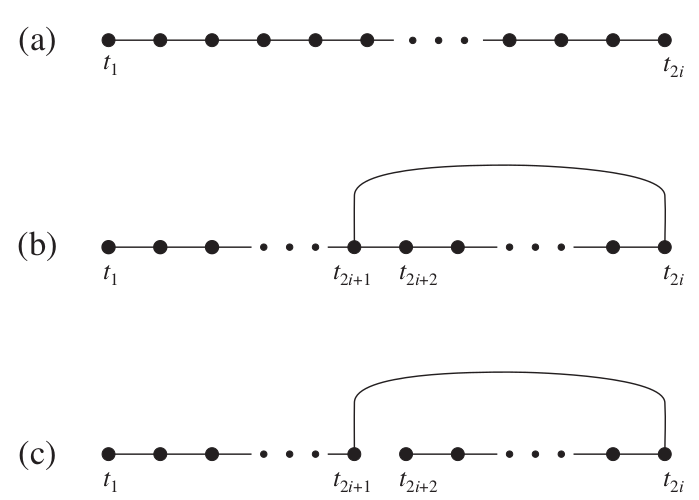
\includegraphics[width=300px]{img/lin_kernighan_move}
    \caption{A Lin-Kernighan move\label{fig:kernig}}
  \end{figure}
  \begin{itemize}
    \item Den er baseret til at subset af 2-opt valg
    \item \textbf{Ancor} af den nuværende path er en fixed slut by $t_1$
    \item Lad $t_{2i}$ være den anden ende af path $P_i$, der eksistere i step $i$ af LK search
    \item Den nuværende tour for den nuværende path $P_i$ fåes ved at tilføje kanter $t_{2i}, t_1$ 
    \item Kun 2 OPT valg som flipper et suffix af pathen altså valget hvor en af tour kanterner der bliver fjernet er $\{t_1, t_{2i}\}$ se Figur \ref{fig:kernig}
    \item Den nye nabo $t_{2i+1}$ af $t_{2i}$ må være længde af spanning træet plus en kant mindre end længden af den bedste tur ind til videre
    \item Den kan med fordel bruges flere gange for at få et bedre resultat
  \end{itemize}
  \item \textbf{Simulated anealing} 
\begin{figure}[ht]
  \centering
\begin{lstlisting}  
Generer en start løsning $S$
Sæt den initiellle bedste løsning $S^* = S$ 
Find ud af en start temperatur $T$
while not fronzen gør følgende 
  while not at equilibrium
    Vælg en random neighbour $S'$
    Sæt $\Delta = Length(S') - Length(S)$
    if $\Delta \leq 0$
      Sæt $S=S'$
      if $Length(S) < Length (S^* )$ sæt $S^* = S$  
    else 
      Vælg et random tal $r$ uniformt i $[0,1]$
      Hvis $r < e^{-\Delta/T}$ sæt $S=S'$
  Gør temperaturen $R$ lavere
return $S^* $
\end{lstlisting}
  \caption{Simulated anealing algoritme\label{fig:simulated-anealing}}
\end{figure}
  \begin{itemize}
  	\item Algoritmen kan ses på Figur \ref{fig:simulated-anealing}
    \item Hvis man gør temperaturen lavere i en rate af $C/\log n$ hvor $n$ er antallet af steps finder den optimale værdi, det er dog meget langsommere end exhaustive search 
    \item Temperaturen bliver typisk gjort lavere meget hurtigere, hvilket giver en approximationsalgoritme
  \end{itemize}
  \item \textbf{Evolutionary algortime} 
\begin{figure}[ht]
  \centering
\begin{lstlisting}  
Generere en population af $k$ start løsninger $S=\{S_1, \dots, S_k\}$
Brug en lokal optimeringsalgoritme $A$ til at løsningerne $S$ i $S$
lad den resulterende løsning erstatte $S$ 
while not converged
  Vælg $k'$ distincte subsets af $S$ af størrelse 1 eller 2 som Forældre
  for hver 1 elements subset udfør en tilfældig mutation for at få en ny løsning 
  for hver 2 elements subset udfør en crossover operation for at få en ny løsning 
  Brug $A$ på hver af de $k'$ løsninger produceret
  lad $S'$ være de resulterende løsninger
  En selection strategi bliver brugt til at vælge $k$ løsninger fra $S \cup S'$
return best solution fra $S$  
\end{lstlisting}
  \caption{Genetisk optimeringsalgoritme\label{fig:evolutionary}}
\end{figure}
  \begin{itemize}
  	\item En generel evolutionel algoritme er beskrevet på Figur \ref{fig:evolutionary}
  \end{itemize}
\end{itemize}

\newpage
%%% Local Variables:
%%% mode: latex
%%% TeX-master: "optimering-noter"
%%% End:
